\iffalse

MIT License

Copyright (c) 2023 Aron Hardeman

Permission is hereby granted, free of charge, to any person obtaining a copy
of this software and associated documentation files (the "Software"), to deal
in the Software without restriction, including without limitation the rights
to use, copy, modify, merge, publish, distribute, sublicense, and/or sell
copies of the Software, and to permit persons to whom the Software is
furnished to do so, subject to the following conditions:

The above copyright notice and this permission notice shall be included in all
copies or substantial portions of the Software.

THE SOFTWARE IS PROVIDED "AS IS", WITHOUT WARRANTY OF ANY KIND, EXPRESS OR
IMPLIED, INCLUDING BUT NOT LIMITED TO THE WARRANTIES OF MERCHANTABILITY,
FITNESS FOR A PARTICULAR PURPOSE AND NONINFRINGEMENT. IN NO EVENT SHALL THE
AUTHORS OR COPYRIGHT HOLDERS BE LIABLE FOR ANY CLAIM, DAMAGES OR OTHER
LIABILITY, WHETHER IN AN ACTION OF CONTRACT, TORT OR OTHERWISE, ARISING FROM,
OUT OF OR IN CONNECTION WITH THE SOFTWARE OR THE USE OR OTHER DEALINGS IN THE
SOFTWARE.

\fi
\section{Taylor polynomials}
\tableofcontents[currentsection,currentsubsection]
\begin{frame}{Taylor polynomials}
    Sometimes, we want to approximate a function by a polynomial.

    The $n$th degree \emph{Taylor polynomial} of function $f$ at $x=a$ is given by
    \pause\[T_n(x)=\sum_{j=0}^n\frac{f^{(j)}(a)}{j!}(x-a)^j,\]
    provided $f$ is differentiable $n$ times.

    \pause\color{gray}This definition has been chosen such that the $i$th derivatives of $f$ are equal to the $i$th derivatives of $T_n(x)$ for $i\in\{0,1,\dots,n\}$. Intuitively, this ensures that around $x=a$, the behavior of the polynomial is similar to the behavior of $f$, i.e., the polynomial \emph{approximates} $f$.
\end{frame}

\begin{frame}
\frametitle{Visualization}
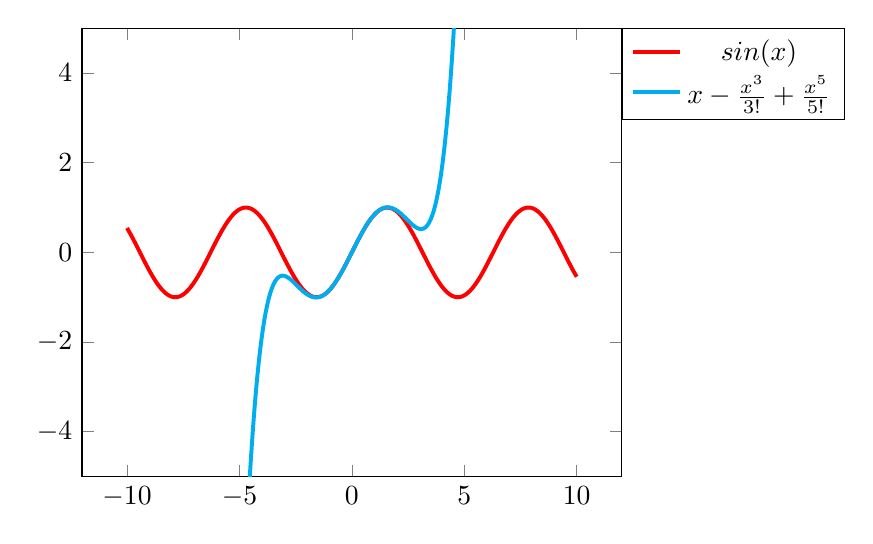
\begin{tikzpicture}
\begin{axis}[legend style={at={(1,1)},anchor=north west},ymin=-5, ymax=5]
\addplot[line width=0.5mm,color=red, domain=-10:10, samples=500]{sin(deg(x))};
\addlegendentry{\(sin(x)\)}
%\addplot[color=blue, domain=-10:10, samples=500]{x};
%\addlegendentry{\(x\)}
%\addplot[color=green, domain=-10:10, samples=500]{x-((x^3)/(3!))};
%\addlegendentry{\(x-\frac{x^3}{3!}\)}
\addplot[line width=0.5mm,color=cyan, domain=-5:5, samples=500]{x-((x^3)/(3!))+((x^5)/(5!))};
\addlegendentry{\(x-\frac{x^3}{3!}+\frac{x^5}{5!}\)}
%\addplot[color=black, domain=-7:7, samples=500]{x-((x^3)/(3!))+((x^5)/(5!))-((x^7)/(7!))};
%\addlegendentry{\(\mathsmaller{{x-\frac{x^3}{3!}+\frac{x^5}{5!}-\frac{x^7}{7!}}}\)}
\end{axis}
\end{tikzpicture}

{ Interactive version: \url{https://www.desmos.com/calculator/elb2sjyuhu}}
\end{frame}


\begin{frame}
\frametitle{Example Taylor polynomial question}
{\scriptsize
    Find an expression for the $(2n+1)$th degree Taylor polynomial $T_{2n+1}(x)$ of the function $f(x)=\sin x$ centered around $x=0$.

------------------------------------------------------------------------------

\pause
Solution: let's compute some derivatives:
\[f^{(0)}(x)=f(x)=\sin x\quad\quad\quad\quad f^{(0)}(0)=0\]
\vspace*{-\baselineskip}\pause\[f^{(1)}(x)=\cos x\quad\quad\quad\quad f^{(1)}(0)=1\]
\vspace*{-\baselineskip}\pause\[f^{(2)}(x)=-\sin x\quad\quad\quad\quad f^{(2)}(0)=0\]
\vspace*{-\baselineskip}\pause\[f^{(3)}(x)=-\cos x\quad\quad\quad\quad f^{(3)}(0)=-1\]
\vspace*{-\baselineskip}\pause\[f^{(4)}(x)=\sin x\quad\quad\quad\quad f^{(4)}(0)=0\]
\vspace*{-\baselineskip}\pause\[f^{(5)}(x)=\cos x\quad\quad\quad\quad f^{(5)}(0)=1\]

\pause We see a pattern! These derivatives will infinitely repeat in a cycle of length four. Using the definition, we get
\begin{flalign*}T_{2n+1}(x)&=\sum_{j=0}^{2n+1}\frac{f^{(j)}(a)}{j!}(x-a)^j=\sum_{j=0}^{2n+1}\frac{f^{(j)}(0)}{j!}x^j\\
    &=x-\frac{x^3}{3!}+\frac{x^5}{5!}-\dots+(-1)^n\frac{x^{2n+1}}{(2n+1)!}=\boxed{\sum_{i=0}^{n}\frac{(-1)^ix^{2i+1}}{(2i+1)!}}.
\end{flalign*}

}
\end{frame}

\begin{frame}{Evaluating limits with Taylor polynomials}
    \begingroup
    \scriptsize
    We can do some nice things with Taylor polynomials, such as evaluating limits.

    \begin{itemize}
        \pause\item \textbf{Question}: evaluate $\displaystyle\lim_{x\to0}\frac{(\sin\sqrt x)^2-x\cos x+\frac13x^2}{x\ln(1+x)-x^2}.$
        \pause\item \textbf{Solution}: replace some of the terms by their Taylor polynomial:
    \end{itemize}
    \vspace{-3mm}
            \begin{flalign*}
                \lim_{x\to0}&\frac{{\color{red}(\sin\sqrt x)^2}-{\color{blue}x\cos x}+\frac13x^2}{\color{teal!30!green}x\ln(1+x)\color{black}-x^2}\\
                            &\action<+->{=\lim_{x\to0}\frac{{\color{red}\left[x^{1/2}-\frac{x^{3/2}}{3!}+\frac{x^{5/2}}{5!}+O(x^{7/2})\right]^2}-{\color{blue}x\left[1-\frac{x^2}{2!}+O(x^4)\right]}+\frac13x^2}{\color{teal!30!green}x\left[x-\frac{x^2}2+O(x^3)\right]\color{black}-x^2}}\\
                            %&\qquad\color{orange}\text{(do this step on the board)}\\
                             &\action<+->{=\lim_{x\to0}\frac{{\color{red}\left[x-\frac13 x^2+(\frac1{3!3!}+\frac{2}{5!})x^3+O(x^4)\right]}-{\color{blue}\left[x-\frac{x^3}{2!}+O(x^5)\right]}+\frac13x^2}{{\color{teal!30!green}\left[x^2-\frac{x^3}2+O(x^4)\right]}-x^2}}\\
                             &\action<+->{=\lim_{x\to0}\frac{(\frac1{3!3!}+\frac{2}{5!}+\frac1{2!})x^3+O(x^4)}{-\frac{1}2x^3+O(x^4)}=}\action<+->{\lim_{x\to0}\frac{\frac{49}{90}+O(x)}{-\frac12+O(x)}=}\action<+->{\frac{\frac{49}{90}+0}{-\frac12+0}=}\action<+->{\boxed{-\frac{49}{45}}}.
            \end{flalign*}
        \textbf{Note: in a similar fashion, you can approximate integrals using Taylor polynomials.}
    \endgroup
\end{frame}

\begin{frame}{Taylor's theorem}
    \begingroup
    \small
    Let us write $f(x) = T_n(x) + E_n(x)$, where $T_n(x)$ is the $n$th degree Taylor polynomial of the function $f$ around $x=a$. We call $E_n(x)$ the \emph{error term}.

    \pause
    \begin{tcolorbox}[title=Taylor's theorem ,colback=yellow!50,colframe=violet!85!black]
    If $f$ is $n+1$ times differentiable on the open interval between $a$ and $x$ and $f^{(n)}$ is continuous on the closed interval between $a$ and $x$, then
    \[E_n(x)=\frac{f^{(n+1)}(c)}{(n+1)!}(x-a)^{n+1}\]
    for some $c$ between $a$ and $x$.
    \end{tcolorbox}
    \pause
    Error estimation theorem (corollary): if there is a positive constant $M$ for which $|f^{(n+1)}(y)|\leq M$ for all $y$ between $a$ and $x$, then
    \[|E_n(x)|\leq \frac{M|x-a|^{n+1}}{(n+1)!}.\]
    \endgroup
\end{frame}

\begin{frame}{Error estimation using Taylor's theorem}
    \textbf{Question}: estimate $\sin(1^\circ)$ with an error less than $10^{-18}$.

    \vspace{2mm}
    \pause
    \textbf{Solution}: 
    \begin{itemize}
        \pause\item We want to approximate $\sin(1^\circ)=\sin\frac1{360}$ using the Taylor polynomials of $\sin x$ (centered around $x=0$). So, for which $n$ do we have $|E_n(\frac1{360})|<10^{-18}$?

        \pause\item By the Error estimation theorem with $M=1$ (why?), we find that $|E_n(\frac1{360})|<10^{-18}$ whenever $\frac{(\frac1{360})^{n+1}}{(n+1)!}<10^{-18}$. This holds for $n\geq5$.

        \pause\item Hence, it suffices to use the Taylor polynomial of degree $5$. We get
            {\footnotesize\[\sin(1^\circ)\approx (1/360)-\frac{(1/360)^3}6+\frac{(1/360)^5}{120}={\color{green!70!teal}0.002777774205534071}367988\dots\]}

        \pause\item Verification: {\footnotesize$\sin(\frac1{360})={\color{green!70!teal}0.002777774205534071}367734\dots$}
        
            \pause
            Verdict: success!

        \end{itemize}
    
\end{frame}





